\section{Literature Review and Theory}
% Delete the text and write your Theory/ Background Information here:
%------------------------------------
\subsection{Current State of the art for UAM}
There exists 2 main approaches for controls of unmanned aerial manipulators: The first one is the centralized approach where we consider the manipulator and the UAV as a whole whereas the decentralized apporach the manipulator control and UAV control are independant problems.
In the case of the Sensor placemen with a quadcopter, we use the centralized approach because the arm has no degree of freedom and the force exerted by the tip is coming from the thrust of the UAV.
The centralized approach is often built on top of a model-based full state control loop optimized with LQR around some desired state. 
In \cite{ruggiero2018aerial}, the author present the current state of the research for UAMs.
An UAM can be divided into 4 elements: The UAV floating base (in our case, a quadcopter), the robotic arm, a sensor/gripper attached to the end of the arm (in our case, a sensor will be attached to the end of the arm), diverse sensors on UAV to handle perception (the depth camera )
\subsection{Velocity field path-planning for single and multiple unmanned aerial vehicles}
In \cite{farinha2020unmanned}, the author presents a path-planning technique based on velocity fields generated from potentials solution of Laplace's equation.
Two different types of solution to potential $V$ for the Laplace 
\begin{align} % Use & sign to align, use \nonumber to write a line without number.
    \laplacian{V} &=0 \nonumber \\
    \frac{\partial^2 V}{\partial x^2}+\dpd[2]{V}{y} &=0 \label{eq:Laplace} % dpd = display mode partial derivative
\end{align}
equation are presented in this paper: Type 1 are irrotational solutions to generate sink and source fields and Type 2 solutions are used to build solenoidal fields.
\begin{align} % Use & sign to align, use \nonumber to write a line without number.
    {V}_{1} = {Q}_{1} \ln(({x}_{1}-\tilde{{x}_{1}})^2+({x}_{2}-\tilde{{x}_{2}})^2) \\
    {V}_{2} = {Q}_{2} \arctan(\frac{({x}_{2}-\tilde{{x}_{2}})}{({x}_{1}-\tilde{{x}_{1}})})
\end{align}
where $({x}_{1},{x}_{2})$ is the position of the UAV, $(\tilde{{x}_{1}}, \tilde{{x}_{2}})$ is the position of the obstacle;
${V}_{1}$ and ${V}_{2}$ are respectively type 1 solution (source field) and type 2 solution (vortex field). \\
The author justifies the use of Laplace solution for building the velocity field for multiple reasons:
\begin{itemize}
    \item The use of Laplace solution for potential guarantees the uniqueness of the minimum in the field. 
    Specifically, the use of vortex function built from shaping function to circle around obstacle will
    ensure that only the goal point will be a minimum of the field and that the UAV will not get stuck at some local minimum. 
    As the author states, we can do an analogy with a famous strategy to find the exit of a maze: 
    by keeping a hand on a wall of the maze and walking while always touching the wall, we are ensured to find the end of the maze. 
    This is far from being an optimal solution, however, it can guarantee that the goal will be reached. 
    As a result, those solenoidal fields based on vortex function also provide active collision avoidance. 
    \item Scalar shaping functions are at the base of these methodology because by crafting them to match the shape of the obstacles, 
    we are able to generate corresponding vortex functions for obstacles of any shape. 
    Since the vortex field is defined for each obstacle, it would be easy to reevaluate the field after addition or removal of an obstacle.
    \item Finally, irrotational solutions of the Laplace equation allow us to enforce an exclusion radius around obstacles (source field) and to direct the UAV in direction of the target point (sink field).
    The exclusion radius is encoded using the amplitude ${Q}_{1}$ of the irrotational field.
\end{itemize}

We can leverage these both types of potentials to derive a velocity field that will guide the UAV to the contact point without colliding with the surface.
For example, we could define the exclusion radius to be the distance between the centre of mass (CoM) of the quadcopter and its most distant part on the quadcopter. 
We will still be able to make contact because the distance between the tip of the arm and the CoM will be longer than this exclusion radius. 


\subsection{Spherical field to maintain desired force }
When contact has been made, we suppose that the surface static friction coefficient is high enough to maintain the contact.
Since the arm has a fixed size and does not move, this section will describe a velocity field on the surface of a sphere around the target point with a radius defined by the distance between the CoM of the quadcopter and the tip of the arm.\\
First we need to compute the feasible position of the CoM to apply the desired force. 
We know that this position is unique because there is only one vertically stable pitch for a given desired force amplitude. The quadcopter needs to pitch to have a forward velocity because the quadcopter is underactuacted.\\
We can either compute this position analytically or we can use machine learning techniques such as regression to compute the feasible pitch as a function of the desired force. The latter option would require collecting training data from simulations on Gazebo. 
Now we can generate the velocity field on the surface of the sphere to point on the tangent direction of the sphere in the direction of the stable pitch position. \\
This field will have an amplitude proportional to the distance from this point.
The planning strategy we described would also allow us to easily define a desirable range for the yaw angle depending on the type of sensor and on the friction coefficient of the target surface.
Finally, we use a Passive Velocity Field Controller \cite{li1999passive} to follow this field to minimize the loss of kinetic energy to the environment when interacting with the surface.

\subsection{Passive Velocity Field Control of Mechanical Manipulators}
In \cite{li1999passive}, the author explains the advantages of encoding a contour following task using velocity fields. 
He later presents the passive velocity field controller whose objective is to "maintain an energetically passive relation-ship between the manipulator under closed loop control and
its physical environment, while causing the manipulator to perform the desired task." 
We will explain each one of those arguments and relate them to our sensor placement task.
\subsubsection{Velocity fields for planning}
The classical approach to do planning is to encode the task into a timed trajectory $Q:\mathbb R_{\ge 0} \rightarrow G$ where G is the n-dimensional configuration manifold for the manipulator.
Using this strategy, the objective of the controller is to minimize the deviation between $q(t)$ and $Q(t)$ where $q:\mathbb R_{\ge 0} \rightarrow G$ is the actual coordinate representation of the manipulator.
This strategy could be fine if the manipulator was able to never deviate from the timed trajectory defined by Q. However, this is rarely the case and when a deviation occurs, a side effect of this minimization strategy called radial reduction can occur.
\begin{figure}[h!]
    \centering
    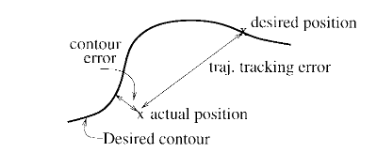
\includegraphics[width=0.48\textwidth]{Images/radialreduction.png}
    \caption{radial reduction from \cite{li1999passive}}
    \label{fig:radialreduction}
\end{figure} 
The author argues that if following the path of the desired trajectory is more important than the timing in which the manipulator follows this trajectory, a strategy based on velocity field is more appropriate because the velocity of the manipulator will only depend on its current position and will be time invariant.  
For the sensor placement task, using a timed trajectory strategy with deviation minimization to reach the contact point may lead the UAV to collide with an obstacle. With our strategy based on potential velocity field, the UAV will not try to shortcut the desired path in case of deviation.

\subsubsection{Passive velocity field controller}
The controller presented in this paper allows storing kinetic energy of the manipulator's actuators in a spring or a flywheel and releasing it when needed so that we can interact with surfaces while minimizing energy loss. This is useful because the UAV has a limited amount of energy stored in its battery and this is one of the main limiting factors for most tasks (including Sensor Placement). \\
To present this concept, the author first define the notion of a passive dynamic system:\\
A dynamic system with input $u \in U$ and output $y \in Y$ is passive with respect to the supply rate 
$s:U \cross Y \rightarrow \mathbb R$, if for any $u: \mathbb R_{\ge 0} \rightarrow U $ and for any $t\geq 0$ the following relation is satisfied:
\begin{align}
    \exists ~ c\in\mathbb R  \nonumber\\
    \int_{0}^{t}s(u(\tau),y(\tau))d\tau \geq -c^2
\end{align}
This supply rate can be seen as the total mechanical power input: $s(\tau_{tot}^{T}\dot{q})$. Here the input $\tau_{tot}$ is the total force exerted on the manipulator 
and $\dot{q}$ is the velocity of the manipulator.
When considering a feedback system interacting with the environement shown in figure \ref{fig:pvfccontrolloop}, we can decompose $\tau_{tot}=\tau_{e}+\tau$ (where $\tau$ and $\tau_{e}$ are respectively the forces generated by the actuators and the external forces, for example the contact force when touching a surface),
we can derive the power generated by external forces as $s(\tau_{e}\dot{q})=\tau_{e}^T \dot{q}$. 
\begin{figure}[h!]
    \centering
    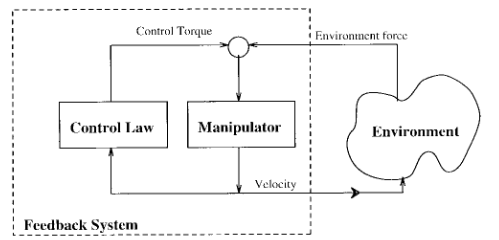
\includegraphics[width=0.48\textwidth]{Images/pvfccontrolloop.png}
    \caption{PVFC loop \cite{li1999passive}}
    \label{fig:pvfccontrolloop}
\end{figure} 
As explained in the paper, a system defined by this supply rate is not passive because obstacles may bring the manipulator to a complete stop for an unbounded amount of time and this loss of kinetic enery cannot be bounded. 
As a result, the passivity relation 
\begin{equation}
    \int_{0}^{t}\tau_{e}^T \dot{q}d\tau \geq -c^2 
\end{equation}
is not valid here because the l.h.s represents the total amount of energy lost to the environment and, as stated before, it cannot be bounded. 
This issue motivates the introduction of an augmented system: a fictitious flywheel is added to the system that acts as an energy storage element.
The dimensionality of the manifold is then increased by one to include the state of the flywheel and this augmented state will be noted as
\begin{equation} 
    \bar{q}=[q_1,...,q_n,q_{n+1}]
\end{equation}
The paper later presents the dynamics of this augmented state and designs a field for the fictitious flywheel such that "the kinetic energy of the augmented system remains constant"